\subsection{OpenID Connect}

O OpenID Connect (OIDC) é um protocolo para fornecimento de identificação que permite que dados de 
usuários sejam transmitidos de forma segura de um provedor para um cliente, com o consentimento do
usuário. É uma camada sobre o protocolo OAuth 2.0, fazendo uso de todos seus conceitos, 
\emph{tokens} e fluxos, com a adição do fornecimento de atributos do usuário. Esses atributos 
podem ser fornecidos para um sistema por meio de uma API RESTful \texttt{userinfo} ou por meio de 
um \emph{token} de identificação \cite{BIEHL2019}.

O fluxo de código de autorização do OIDC é similar ao fluxo do OAuth 2.0, com a adição do 
\emph{token} de identificação, fornecido ao cliente pelo servidor de autorização (chamado de 
provedor OIDC). Este \emph{token} é no formato JWT e possui declarações sobre a autenticação
de um usuário (Figura \ref{fig:OpenID}). Estas declarações também podem ser acessadas realizando uma 
requisição ao \emph{endpoint} \texttt{userinfo} \cite{OIDCCORE}. 

% O OpenID Connect (OIDC) é um padrão de camada de identificação em cima do protocolo OAuth 2.0. Utiliza 
% todos os conceitos, \emph{tokens} e fluxos do protocolo OAuth 2.0, com a adição do fornecimento de 
% atributos do usuário. Esses atributos podem ser 
% fornecidos para um sistema por meio de uma API RESTful \texttt{userinfo} ou por meio de um 
% \emph{token} de identificação \cite{BIEHL2019}.

% O OIDC implementa autenticação como uma extensão da autorização fornecida pelo protocolo OAuth 2.0.
% Seu fluxo de código de autorização é similar, com o OIDC possuindo a adição do 
% \emph{token} de autenticação, fornecido ao cliente pelo servidor de autorização (chamado de 
% provedor OIDC). Este \emph{token} é no formato JWT e possui declarações sobre a autenticação
% de um usuário (Figura \ref{fig:OpenID}). Estas declarações também podem ser acessadas realizando uma 
% requisição ao \emph{endpoint} \texttt{userinfo} \cite{OIDCCORE}.

% \begin{itemize}
%     \item O cliente (sistema solicitando acesso) redireciona para o servidor de autenticação 
% (Provedor OIDC) com os parâmetros necessários (ID do cliente, URI de redirecionamento, etc.);
%     \item O provedor apresenta uma página de login ao usuário;
%     \item Após login bem sucedido, é solicitada a permissão de acesso aos recursos para o usuário;
%     \item O provedor OIDC redireciona o usuário ao cliente, com o código de autorização;
%     \item O cliente solicita ao provedor OIDC um \emph{token} de identificação e também geralmente
% \emph{tokens} de acesso e atualização;
%     \item O provedor envia ao cliente os \emph{tokens} que podem ser utilizados para acessar 
% informações do usuário (\emph{endpoint} \texttt{userinfo}), recursos protegidos e solicitar novos 
% \emph{tokens} \cite{OIDCCORE}.
% \end{itemize}

\begin{figure}[ht]
    \centering
    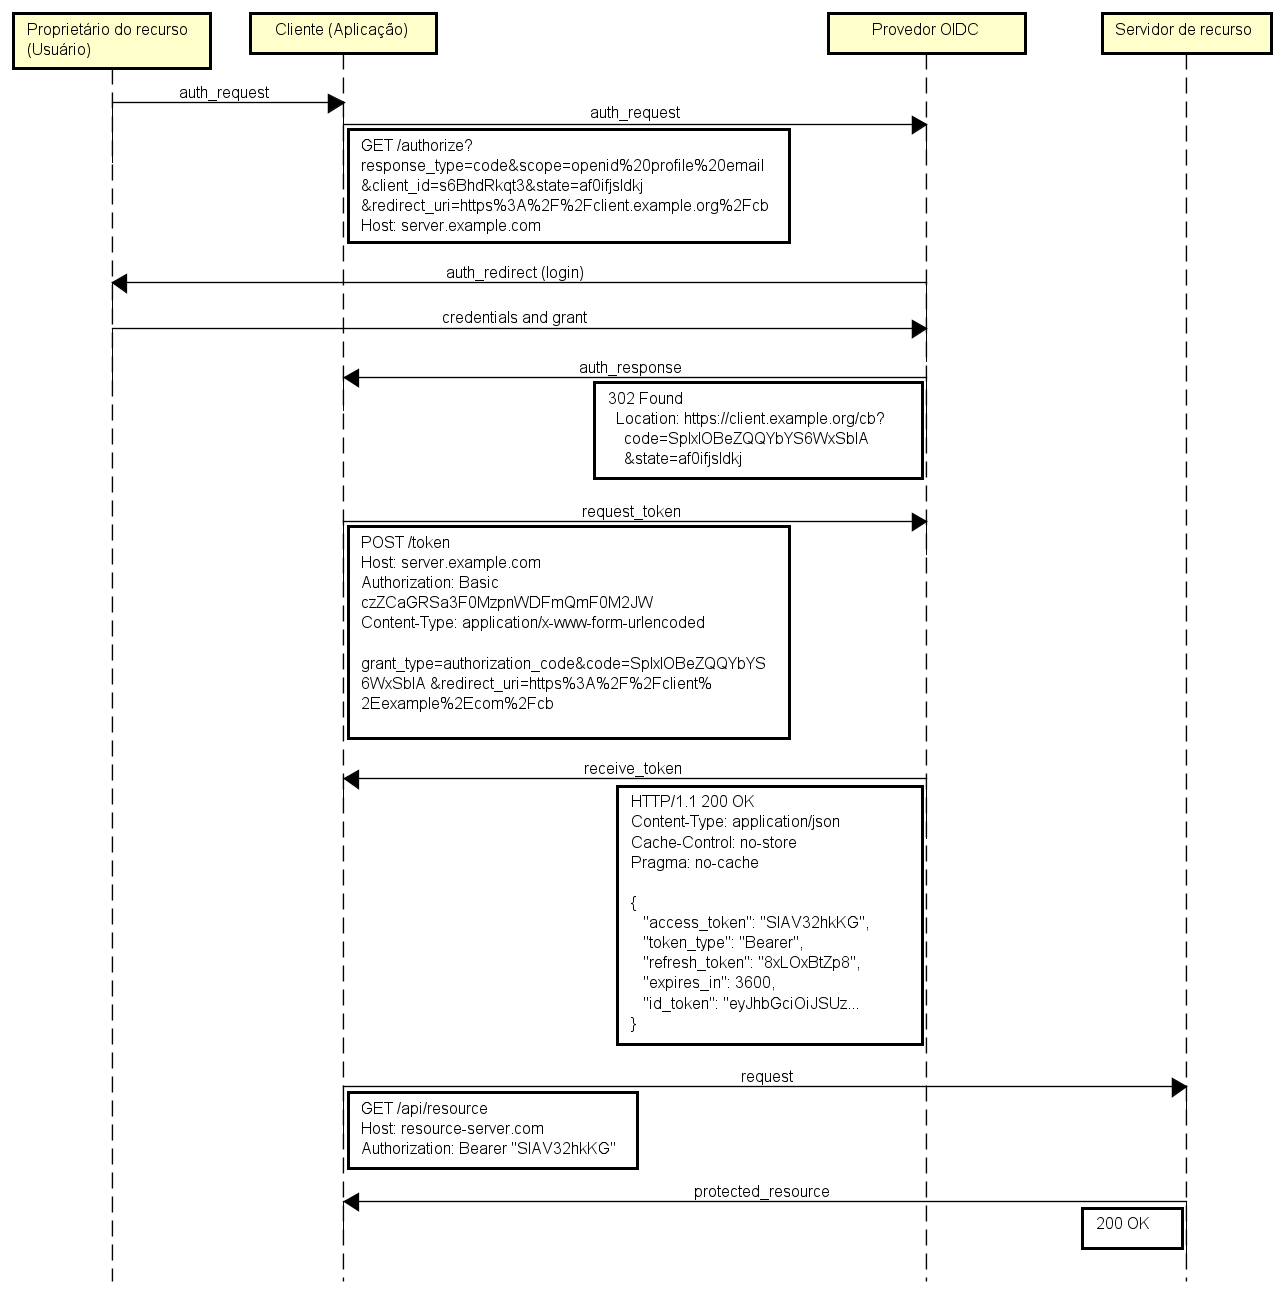
\includegraphics[width=.95\textwidth]{OpenID Connect.png}
    \caption{Exemplo de autenticação utilizando OpenID Connect.}
    \label{fig:OpenID}
\end{figure}